\scanpage{21}

\mspage{42}

on trouve une suite exacte canonique \inserted{(où $Z_\ell[1]=\varprojlim_\nu\deleted{Z}\mu_{\ell^\nu}$ est le faisceau $\ell$-adique de TATE)}:
\diagram{\begin{tikzcd}[ampersand replacement=\&,column sep=small]
(8.3)\quad0\arrow[r]\&t^{i-1}(X,\ell)\arrow[r]\&H^i(X,\uline Z_\ell[1])\arrow[r]\&T_\ell(H^i(X,\mu_{\ell^\infty}))\arrow[r]\&0,
\end{tikzcd}}
où \deleted{$\unsure{t^{i-1}(X,\ell)}$} on a posé
\[
(8.4)\qquad t^{i-1}(X,\ell)=H^{i-1}(X,\mu_{\ell^\infty})/H^{i-1}(X,\mu_{\ell^\infty})^0
\]
qui est donc un groupe fini de $\ell$-torsion, et s'identifie donc, par (8.3), au sous-\deleted{groupe}\inserted{module} de torsion de $\uline Z_\ell$-module de type fini
\[
(8.5)\qquad H^i(X,\uline Z_\ell[1])=\lim H^i(X,\mu_{\ell^\nu}\deleted{\unsure{\ell^\nu Z}}),
\]
dont la partie libre s'identifie, à son tour, à $T_\ell(H^i(X,\mu_{\ell^\infty}))$. On en déduit également un isomorphisme
\[
(8.6)\qquad \deleted{\unsure{T}}(H^i(X,\mu_{\ell^\infty})^0\simeq H^i(X,\uline Z_\ell[1])\otimes_{\uline Z_\ell}\uline Q_\ell/\operatorname{Im}H^i(X,\uline Z_\ell[1]),
\]
qui montre que $H^i(X,\mu_{\ell^\infty})$ et $H^i(X,\uline Z_\ell[1])$ se déterminent mutuellement mod groupes \deleted{\unsure{dant|d'ordre}} finis.

\inserted{8.2.} Un passage à la limite analogue dans \deleted{les suites exactes}\inserted{la suite exacte} de Kummer (BR II 3.1) nous donne de même une suite exacte
\diagram{\begin{tikzcd}[ampersand replacement=\&,column sep=small]
(8.7)\quad0\arrow[r]\&\operatorname{NS}(X)\otimes_{\uline Z}\uline Z_\ell\arrow[r]\&H^2(X,\uline Z_\ell[1])\arrow[r]\&T_\ell(\operatorname{Br}'(X))\arrow[r]\&0,
\end{tikzcd}}
en supposant maintenant que $\operatorname{Pic}(X)$ est extension d'un groupe de type fini $\operatorname{NS}(X)$ (le \uline{groupe de Néron--Sévéri}) par un groupe divisible, et que $H^2(X,\uline Z/\ell\uline Z)$ est fini. \deleted{\unsure{x}}On trouve en passant le fait, classique dans la théorie transcendante, que \deleted{le}\inserted{\figure{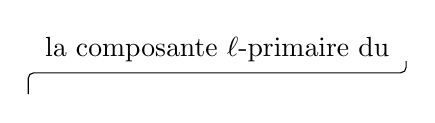
\begin{tikzpicture}
\node at(0,0){la composante $\ell$-primaire du};
\draw[rounded corners=2pt](-2.4,-.57)--(-2.4,-.3)--(2.4,-.3)--(2.4,-.15);
\end{tikzpicture}}} sous-groupe de torsion de $\operatorname{NS}(X)$ est isomorphe au sous-groupe de torsion de $H^2(X,\uline Z_\ell[1])$, en même temps qu'on précise du point de vue de la cohomologie $\ell$-adique la relation entre le groupe de Brauer (ou plus précisément, $T_\ell(\operatorname{Br}'(X))$) et la ``partie transcendante'' du $H^2$, \deleted{\unsure{x}}comparer (BR II 3 passim).

Lorsque $X$ est \inserted{\figure{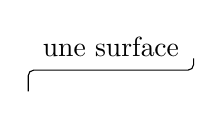
\begin{tikzpicture}
\node at(0,0){une surface};
\draw[rounded corners=2pt](-1.05,-.57)--(-1.05,-.3)--(1.05,-.3)--(1.05,-.15);
\end{tikzpicture}}} propre, lisse et connexe sur un corps $k$ algébriquement clos, il y a lieu de considérer sur le terme médian de (8.7) la forme bilinéaire symétrique canonique, fournie par le cup-produit,\deleted{\unsure{à|x}} qui est à valeurs dans

\mspage{20}
